\subsection{Vertex Cover (VC)}
Given a graph $G=(V,E)$, a vertex cover is a subset $S \subseteq V$, so that for each edge $(u,v) \in E$ at least one of $u$ or $v$ lies in $S$.

Vertex cover decision problem (VC):
\begin{itemize} 
	\item Instance: graph $G$, integer $k$
	\item Question: does $G$ have a vertex cover of size at most $k$?
\end{itemize}

Clearly in NP. The certificate is just the subset of vertices forming the vertex cover. An algorithm can check in polynomial time that the subset is of the right size and that every edge is covered.

\subsection{IS and VC}
Once again, we have a choice of which NP-complete problem to reduce to VC. This time independent set (IS) is the right one. Before we do the reduction, let's understand the relationship between IS and VC. The following example shows that $(V-S)$ is a vertex cover, where $S$ is an independent set. This also holds true in the other direction: if $S$ is a vertex cover then $V-S$ is an independent set.

\begin{figure}[H]
	\centering
	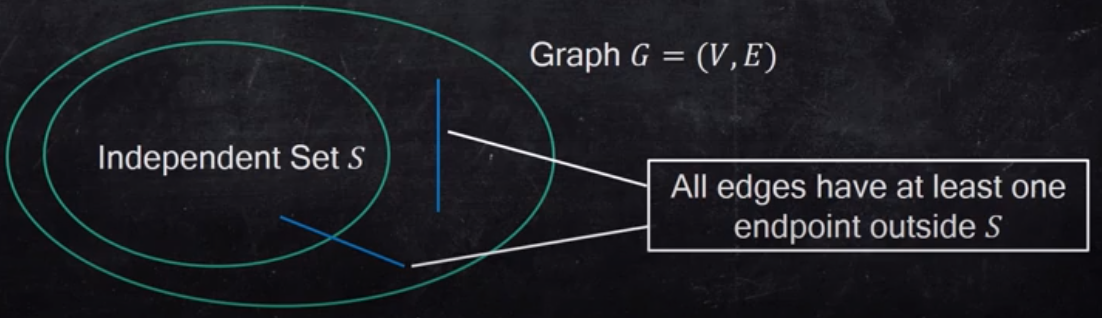
\includegraphics[width=0.5\textwidth]{fig/is-vc.png}
\end{figure}

Thus, a graph with n vertices has an independent set of size at least $k$ if and only if it has a vertex cover of size at most $n-k$.

The reduction is now fairly obvious: Given an instance $\langle G, k \rangle$ of IS, we transform it into an instance $\langle G,n-k \rangle$ of VC.

\subsubsection{Reduction}
If $G$ has an IS, $S$, of size at least $k$, then $V-S$ is a VC of size at most $n-k$. Thus, YES-instances of IS map to YES-instances of VC. If $G$ has a VC, S, of size at most $n-k$, then it has an IS, $V-S$, of size at least $k$. Thus, YES instances of VC map to YES instances of IS. It's easy to see that the reduction runs in poly-time since we are only changing the number.


